\section{Review Methodology}
\label{sec:methodology}

This review follows a structured methodology with transparent reporting of search, screening, and selection. It does not claim formal PRISMA protocol registration.

\subsection{Review Design and Seeds}
The collection is seed-anchored rather than database-exhaustive. Seed 1 (P001) is a comparative experimental study of UAV-based river waste detection that serves as the methodological blueprint (training strategies, UAV datasets, cross-river evaluation) \cite{Pati2025}. Seed 2 (P002) is a systematic review of remote sensing for river macroplastics that provides the state-of-the-art baseline and the backward-tracking corpus \cite{Marye2025}. Two further reviews (P003 on deep learning for macroplastic detection \cite{Jia2023}; P008's companion corpus) and the P004 early river-DL study \cite{Jakovljevic2020} extended the backward-tracking set.

\subsection{Sources Searched}
Backward citation tracking was performed over (i) the base-paper bibliography (\texttt{references.bib}), (ii) the WIREs review evidence tables, and (iii) three connected-paper export files ($\sim$122 titles, deduplicated against the collection). Targeted web retrieval acted as a proxy for Scopus, Web of Science, IEEE Xplore, MDPI, and ScienceDirect across keyword sweeps (river + UAV + deep learning; YOLO river waste; satellite river debris; pond/lake/canal detection; 2024--2026 architectures). No full database keyword pass and no Scholar/Scopus forward tracking were executed; both are recorded as deferred in the search log rather than silently omitted.

\subsection{Scope As Applied}
The working scope --- deep learning and computer vision for waste detection in rivers, ponds, and closely related freshwaters, 2015--2026, peer-reviewed journals and reputable conferences, global coverage with Nepal as guiding context --- describes the corpus as collected rather than gating it: all 50 included studies fall in 2019--2025 and meet the criteria as applied. Preprints and theses were held out regardless of relevance. One low-index venue is retained but cited thinly, and one infrastructure-monitoring study is included as explicitly scoped adjacent work.

\subsection{Screening and Selection}
Over 190 titles were screened and about 75 abstracts or full texts assessed, yielding 50 primary studies (P001, P004--P052) plus two context-only reviews. Around 25 exclusions are documented with reasons (SAR-only sensing, manual-only observation, marine-only or land-only settings, classical non-learning methods, microplastic-only focus, inadequate venue). A quality-control reversal is reported transparently: one provisionally included hyperspectral study was removed after full-text inspection showed land-only model training, restoring the count to 50.

\subsection{Data Extraction and Evidence Grading}
Each study was extracted into a 40-field schema (identifier, bibliographic details, site, platform, spectral range, dataset, task, architecture, training strategy, metrics, limitations, research-question mapping). Generalization claims were graded on a four-level scale: (A) demonstrated cross-environment testing with separate metrics; (B) indirect evidence; (C) author claim without external test; (D) no cross-testing. The corpus grades 20 A, 13 B, 2 C, and 15 D. Cross-environment scope was tagged with an eight-class taxonomy (within-environment; cross-location; cross-platform; cross-dataset; methodological transfer; weight transfer; representation transfer). Provisional rows lacking full-text confirmation are quarantined from strong claims, and preprint-versus-published metric conflicts were resolved in favor of the version of record.

\subsection{Screening Limitations}
Screening was performed by a single extraction agent with human review of decision logs and flags; it was not double-blind. Flow counts below are best-estimate working numbers from the search log, and the selection diagram (Fig.~\ref{fig:prisma}) is an organizational aid, not a compliance statement.
% PRISMA-style selection diagram (organizational aid only; not a compliance statement).
% Numbers are best-estimate working counts from search_protocol/search_log.md (Searches 1--17).
\begin{figure}[!t]
\centering
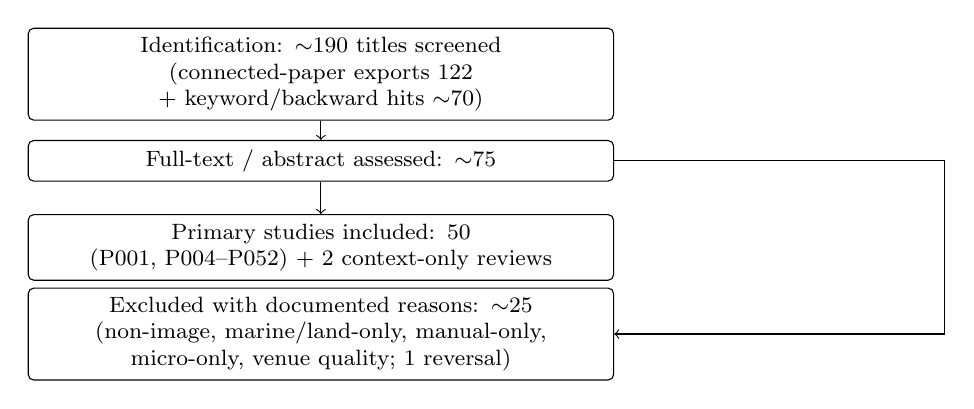
\begin{tikzpicture}[node distance=1.1cm, every node/.style={draw, rounded corners=2pt, text width=7.2cm, align=center, font=\footnotesize}]
\node (id1) {Identification: $\sim$190 titles screened\\(connected-paper exports 122 + keyword/backward hits $\sim$70)};
\node (id2) [below of=id1] {Full-text / abstract assessed: $\sim$75};
\node (inc) [below of=id2] {Primary studies included: 50\\(P001, P004--P052) + 2 context-only reviews};
\node (exc) [below of=inc] {Excluded with documented reasons: $\sim$25\\(non-image, marine/land-only, manual-only,\\micro-only, venue quality; 1 reversal)};
\draw[->] (id1) -- (id2);
\draw[->] (id2) -- (inc);
\draw[->] (id2) -| ([xshift=4.2cm]id2.east) |- (exc);
\end{tikzpicture}
\caption{Selection flow for the review corpus (working counts; single-agent screening with human log review).}
\label{fig:prisma}
\end{figure}

